%% Scaling analysis of one collective family: allgather/bruck
%%
%% generated.tex holds the derived facts and is rewritten by
%%   python3 scripts/analyze_family.py --family allgather/bruck
%% This file is never overwritten: it is where interpretation lives.
\documentclass[11pt]{article}
%% Shared preamble for the per-run AgentMPI analysis documents.
%%
%% One preamble for all of them, so five hundred documents cannot drift into five hundred
%% typographic dialects, and so a change to how findings are marked takes one edit.
%%
%% The severity marks are deliberately words rather than colours alone: these documents are
%% read on screen, printed, and skimmed in diffs, and a colour-only encoding survives none of
%% the last two.

\usepackage[T1]{fontenc}
\usepackage[utf8]{inputenc}
\usepackage{lmodern}
\usepackage[margin=1in]{geometry}
\usepackage{graphicx}
\usepackage{booktabs}
\usepackage{amsmath}
\usepackage{amssymb} % \checkmark, used by the model-agreement marks below
\usepackage{enumitem}
\usepackage{xcolor}
\usepackage{microtype}
\usepackage[hidelinks]{hyperref}
\usepackage{caption}

\captionsetup{font=small,labelfont=bf}
\setlength{\parskip}{0.4em}
\setlength{\parindent}{0pt}

%% Palette lifted from the trace viewer so a document and the dashboard agree on what a colour
%% means. Kept in sync by src/agentmpi/trace_style.py and tests/test_trace_style.py.
\definecolor{ampitrouble}{HTML}{EF4444}
\definecolor{ampiwarn}{HTML}{F59E0B}
\definecolor{ampiok}{HTML}{10B981}
\definecolor{ampinote}{HTML}{60A5FA}
\definecolor{ampimuted}{HTML}{64748B}

\usepackage{xstring}

%% \finding{critical|warning|note|ok} -- a severity tag for a mechanically detected observation.
\newcommand{\finding}[1]{%
  \IfStrEqCase{#1}{%
    {critical}{\textcolor{ampitrouble}{\textbf{[critical]}}}%
    {warning}{\textcolor{ampiwarn}{\textbf{[warning]}}}%
    {note}{\textcolor{ampinote}{\textbf{[note]}}}%
    {ok}{\textcolor{ampiok}{\textbf{[ok]}}}%
  }[\textbf{[#1]}]%
}

%% Verdict marks for the collective/cost-model comparison table.
\newcommand{\modelok}{\textcolor{ampiok}{$\checkmark$}}
\newcommand{\modelbad}{\textcolor{ampitrouble}{$\times$}}
\newcommand{\modelna}{\textcolor{ampimuted}{--}}

%% Unfilled interpretation. Rendered loudly on purpose: an analysis document that ships with
%% its judgement sections empty should be obvious at a glance, not discoverable only by reading.
\newcommand{\TODO}[1]{\textcolor{ampiwarn}{\textbf{[to be written]} \textit{#1}}}


\title{\textbf{allgather/bruck}\\[2pt]\large An AgentMPI collective scaling analysis}
\author{}
\date{}

\begin{document}
\maketitle

\begin{abstract}
Bruck's allgather is the algorithm that gets logarithmic depth at \emph{every} process count
rather than only at powers of two, and it is AgentMPI's default above $p=3$ for exactly that
reason. Each rank keeps the blocks it holds in rotated order, and in round $k$ it sends the first
$\min(2^k,\, p-2^k)$ of them a distance $2^k$ around the circle, doubling its holdings each round
until it has all $p$; one local rotation at the end puts them in rank order. Across 21 process
counts from 2 to 32 the logged traffic matches the closed form $p\lceil\log_2 p\rceil$ messages in
$\lceil\log_2 p\rceil$ rounds at every size, powers of two and otherwise, and the self-report
matches the log at every size. What the family view adds to that unsurprising agreement is why
the $\min(\cdot)$ clamp is there: it makes the number of blocks each rank sends exactly $p-1$ at
every $p$, so the total volume is the information-theoretic floor $p(p-1)n$ and not the
$2^{\lceil\log_2 p\rceil}-1$ an unclamped doubling would send. Bruck therefore attains ring's
optimal volume at ring's $p/\log_2 p$-fold lower round count, which is why ring has no remaining
case. The comparison worth making is the other one. At powers of two Bruck and
\texttt{recursive\_doubling} send the identical number of messages in the identical number of
rounds carrying the identical number of blocks --- 160 messages, 5 rounds, 992 blocks at $p=32$ ---
and differ only in encoding: recursive doubling tags each block with its rank index and Bruck
does not, so recursive doubling puts 6{,}624 tokens on the wire where Bruck puts 3{,}360, and its
largest single message is 106 tokens against Bruck's 53. Bruck runs everywhere and costs half as
much on the wire; recursive doubling runs at nine of twenty-one sizes and costs twice. There is no
regime in this archive where recursive doubling is preferable.
\end{abstract}

% Generated by scripts/analyze_family.py. Do not edit; edit analysis.tex instead.

\section{What this family is}
The \texttt{allgather} collective under the \texttt{bruck} algorithm, measured at 21 process counts from 2 to 32. Every run is agent-free and deterministic, so the measurements are of the protocol itself.

\section{What the analysis notices}
\begin{itemize}[leftmargin=1.4em]
  \item \finding{ok} All 21 measured sizes logged exactly the number of messages the closed form predicts.
  \item \finding{note} Wall times span 0.014--0.273\,s with no agent in the loop, so these measure the fabric and the protocol rather than model latency.
\end{itemize}

\begin{figure}[htbp]
  \centering
  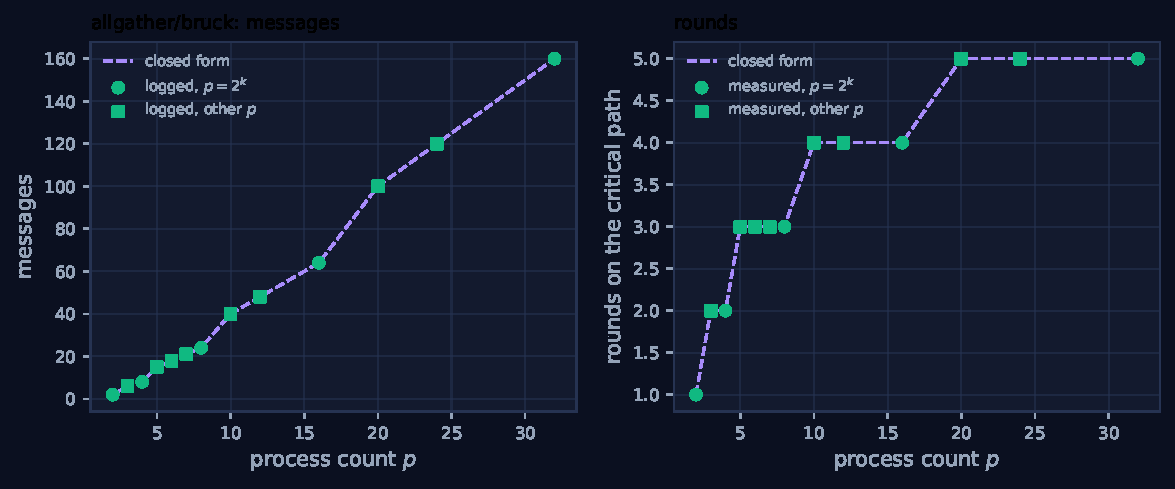
\includegraphics[width=\linewidth]{figures/family.pdf}
  \caption{Measured message count and critical-path rounds against process count, with the closed-form prediction. Powers of two are drawn as circles and other sizes as squares, because algorithms take a different code path at sizes that are not powers of two. A red cross marks a size where the collective's own reported count disagrees with the traffic the fabric logged.}
  \label{fig:family}
\end{figure}

\section{Every measured size}
\begin{center}\footnotesize
\begin{tabular}{@{}rlrrrrrrcc@{}}
\toprule
  $p$ & campaign & logged & pred. & self-rep. & rounds & pred. & wall (s) & model & acct. \\
\midrule
  2 & \texttt{mb-free} & 2 & 2 & 2 & 1 & 1 & 0.015 & \modelok & \modelok \\
  2 & \texttt{mb-smoke} & 2 & 2 & 2 & 1 & 1 & 0.014 & \modelok & \modelok \\
  3 & \texttt{mb-free} & 6 & 6 & 6 & 2 & 2 & 0.016 & \modelok & \modelok \\
  3 & \texttt{mb-smoke} & 6 & 6 & 6 & 2 & 2 & 0.018 & \modelok & \modelok \\
  4 & \texttt{mb-free} & 8 & 8 & 8 & 2 & 2 & 0.020 & \modelok & \modelok \\
  4 & \texttt{mb-smoke} & 8 & 8 & 8 & 2 & 2 & 0.029 & \modelok & \modelok \\
  5 & \texttt{mb-free} & 15 & 15 & 15 & 3 & 3 & 0.037 & \modelok & \modelok \\
  5 & \texttt{mb-smoke} & 15 & 15 & 15 & 3 & 3 & 0.032 & \modelok & \modelok \\
  6 & \texttt{mb-free} & 18 & 18 & 18 & 3 & 3 & 0.035 & \modelok & \modelok \\
  7 & \texttt{mb-free} & 21 & 21 & 21 & 3 & 3 & 0.031 & \modelok & \modelok \\
  7 & \texttt{mb-smoke} & 21 & 21 & 21 & 3 & 3 & 0.071 & \modelok & \modelok \\
  8 & \texttt{mb-free} & 24 & 24 & 24 & 3 & 3 & 0.037 & \modelok & \modelok \\
  8 & \texttt{mb-smoke} & 24 & 24 & 24 & 3 & 3 & 0.052 & \modelok & \modelok \\
  10 & \texttt{mb-free} & 40 & 40 & 40 & 4 & 4 & 0.096 & \modelok & \modelok \\
  12 & \texttt{mb-free} & 48 & 48 & 48 & 4 & 4 & 0.081 & \modelok & \modelok \\
  12 & \texttt{mb-smoke} & 48 & 48 & 48 & 4 & 4 & 0.237 & \modelok & \modelok \\
  16 & \texttt{mb-free} & 64 & 64 & 64 & 4 & 4 & 0.144 & \modelok & \modelok \\
  16 & \texttt{mb-smoke} & 64 & 64 & 64 & 4 & 4 & 0.140 & \modelok & \modelok \\
  20 & \texttt{mb-free} & 100 & 100 & 100 & 5 & 5 & 0.163 & \modelok & \modelok \\
  24 & \texttt{mb-free} & 120 & 120 & 120 & 5 & 5 & 0.273 & \modelok & \modelok \\
  32 & \texttt{mb-free} & 160 & 160 & 160 & 5 & 5 & 0.267 & \modelok & \modelok \\
\bottomrule
\end{tabular}\normalsize
\end{center}



\section{How the algorithm scales}

\subsection{Where the cost comes from}

The awkward thing about a logarithmic allgather is that the natural formulation --- exchange with
the partner at distance $2^k$ and merge --- needs a hypercube, and a hypercube needs $p$ to be a
power of two. Bruck's trick is to give up on holding blocks in the right order until the very end.
Rank $r$ starts with its own block in local slot 0. In round $k$ it sends the first $n_k$ of its
local slots to $(r - 2^k) \bmod p$ and receives the same number from $(r + 2^k) \bmod p$,
appending them; after the last round its local list holds the block of rank $(r+i) \bmod p$ at
slot $i$, and one rotation fixes it up.

Message count follows immediately: one \texttt{sendrecv} per rank per round, so
$p\lceil\log_2 p\rceil$ messages in $\lceil\log_2 p\rceil$ rounds. Rounds are sequential --- round
$k$ sends slots that round $k-1$ filled --- so that is also the critical path.

Volume needs the clamp, and the clamp is the part worth explaining because it is where the
algorithm earns its optimality. Doubling naively would have rank $r$ send $2^k$ slots in round
$k$, giving $\sum_{k<\lceil\log_2 p\rceil} 2^k = 2^{\lceil\log_2 p\rceil} - 1$ blocks per rank ---
which is $p-1$ when $p$ is a power of two and up to nearly $2p$ otherwise. The implementation
instead sends $n_k = \min(2^k,\, p - 2^k)$, and that sum is exactly $p-1$ at every $p$: at $p=10$
it is $1+2+4+2 = 9$; at $p=12$, $1+2+4+4 = 11$; at $p=24$, $1+2+4+8+8 = 23$. The clamp says
``never send a rank a block it will already have'', and the consequence is that Bruck moves
$p(p-1)n$ tokens --- the same floor as ring, since every rank must receive $(p-1)n$ --- rather
than overshooting at non-power-of-two sizes. The \texttt{cost.FORMULAS} entry
$(\lceil\log_2 p\rceil,\, p\lceil\log_2 p\rceil,\, p(p-1)n,\, 0)$ is that derivation.

The log confirms both halves. Grouping the 160 sends of
\texttt{mb-free\_\_coll-allgather-bruck-32} by round gives 32 messages in each of 5 rounds
carrying 4, 7, 14, 27 and 53 tokens --- the doubling sequence, and $1+2+4+8+16 = 31 = p-1$ blocks
per rank once the framing is subtracted. At $p=10$ the four rounds carry $1, 2, 4, 2$ blocks and
the last figure is the clamp firing: $\min(8, 2) = 2$.

\subsection{What the figure shows, and one thing it hides}

The rounds panel of Figure~\ref{fig:family} is the clean $\lceil\log_2 p\rceil$ staircase, with
flat treads at 3 for $p \in [5,8]$, at 4 for $p \in [9,16]$ and at 5 for $p \in [17,32]$, and the
measured points sit on it at all 21 sizes with both marker classes on the same treads. This is
the whole point of choosing Bruck: adding ranks inside a bracket is free in depth, and the depth
grows by one only when the population doubles.

The messages panel looks nearly linear, and it is worth being precise about why it is not. Inside
a bracket the count is $p$ times a constant, so it rises with slope $\lceil\log_2 p\rceil$;
crossing a power of two the slope increments and the value jumps, because $p=16$ costs $16 \cdot 4
= 64$ and $p=17$ costs $17 \cdot 5 = 85$. That is a 33\% increase in traffic for one extra rank,
and it is the single most actionable fact in this family: a harness sized at 16 or 32 ranks is at
a local cost minimum, and one sized at 17 or 33 is not.

The figure does not show that step, and the reason is a property of how it is drawn rather than of
the algorithm. The dashed closed-form line is evaluated only at the measured process counts and
joined by straight segments, so the segment from $p=16$ to $p=20$ interpolates across the
discontinuity at $p=17$ and renders it as a uniform slope of 9 messages per rank. The true
behaviour in that interval is a jump of 21 followed by a slope of 5. The same applies between
$p=8$ and $p=10$, where the plotted slope of 8 conceals a jump of 12 at $p=9$ followed by a slope
of 4. Nothing is wrong with the measurements --- every measured point is exactly on the exact
closed form --- but a reader estimating the marginal cost of one more rank from the line's
gradient will get it wrong near a power of two, in the direction of thinking it smoother than it
is.

There are no red crosses. The self-report matches the logged count at all 21 sizes, which is what
one expects from an algorithm whose accounting is a single \texttt{tr.sent()} in an unbranched
loop --- and which is not what happened in \texttt{allreduce/recursive\_doubling}, whose
accounting had to cover a branch.

\section{Powers of two and everything else}

The two marker classes behave identically, and unlike ring --- which has no size-dependent
behaviour to get right --- Bruck does have one and gets it right.

The size-dependent piece is the clamp, $n_k = \min(2^k,\, p - 2^k)$. It is inactive at powers of
two, where $2^k < p - 2^k$ for every round except the last and the last is $2^{\log_2 p - 1} =
p/2 = p - 2^{\log_2 p - 1}$, a tie. It is active at every other size, and it fires in the final
round or rounds: at $p=10$ the fourth round sends 2 blocks where naive doubling would send 8; at
$p=20$ the fifth sends 4 where doubling would send 16; at $p=24$ the fifth sends 8 where doubling
would send 16. The measured volumes confirm the clamp worked: the reported block totals are
$p(p-1)$ at all 21 sizes --- 90 at $p=10$, 380 at $p=20$, 552 at $p=24$ --- which is what the
clamped sum gives and not what the unclamped one would.

That is the whole remainder story, and it is a good illustration of the difference between an
algorithm that avoids the awkward case and one that handles it. \texttt{allgather/ring} has no
awkward case because modular arithmetic does not have one.
\texttt{allgather/recursive\_doubling} has one and refuses it, falling back to Bruck.
\texttt{allreduce/recursive\_doubling} has one, handles it with a three-phase remainder
correction, and that correction is where the sweep's one real accounting defect lives. Bruck has
one and handles it with a single \texttt{min()} that has no separate code path at all --- no
pre-phase, no renumbering, no branch whose two sides can be instrumented inconsistently. Where
the awkward case can be absorbed into an expression rather than a branch, it should be.

One asymmetry the figure does not distinguish is worth naming. At non-power-of-two sizes the
\emph{message count} still assumes $\lceil\log_2 p\rceil$ full rounds of $p$ messages, so a rank
sends in every round even when the clamp has cut what it sends down to a fraction. At $p=17$ the
fifth round moves one block per rank and still costs 17 messages. The round count is optimal and
the message count is not tight; both match their closed forms, which is all the model claims.

\section{When to choose this algorithm}

\subsection{Against ring: dominant, and by how much}

Both algorithms ran at all 21 sizes on the same payload, so \texttt{mb-free} figures compare
directly:

\begin{center}\footnotesize
\begin{tabular}{@{}rrrrrrrrr@{}}
\toprule
  & \multicolumn{2}{c}{messages} & \multicolumn{2}{c}{rounds} & \multicolumn{2}{c}{wire tokens} & \multicolumn{2}{c}{collective wall (s)} \\
  \cmidrule(r){2-3}\cmidrule(r){4-5}\cmidrule(r){6-7}\cmidrule(r){8-9}
  $p$ & bruck & ring & bruck & ring & bruck & ring & bruck & ring \\
\midrule
  4  & 8   & 12  & 2 & 3  & 44   & 144   & 0.018 & 0.024 \\
  8  & 24  & 56  & 3 & 7  & 200  & 672   & 0.031 & 0.073 \\
  16 & 64  & 240 & 4 & 15 & 832  & 2880  & 0.134 & 0.186 \\
  24 & 120 & 552 & 5 & 23 & 1896 & 6624  & 0.255 & 0.635 \\
  32 & 160 & 992 & 5 & 31 & 3360 & 11904 & 0.225 & 1.131 \\
\bottomrule
\end{tabular}\normalsize
\end{center}

\noindent
At $p=32$: $6.2\times$ fewer messages, $6.2\times$ fewer rounds, $3.5\times$ fewer wire tokens,
$5\times$ less wall clock. There is no size at which ring leads on any of these columns, and at
$p=2$ and $p=3$, where messages and rounds tie, Bruck is still $3\times$ cheaper on the wire.

Two honest deductions from that. The wire-token advantage is largely framing at this benchmark's
one-token blocks --- ring pays an 11-token envelope on each of $p(p-1)$ messages while Bruck
amortises one envelope over up to $p/2$ blocks --- and it would shrink to under 1\% at a
1200-token payload, where \texttt{cost.predict} gives both algorithms the same \$3.5712 at
$p=32$. The wall-clock advantage is inflated by the receive-side poll backoff, which penalises
ring's 31-deep critical path much more than Bruck's 5-deep one. What survives both deductions is
the round count, and \texttt{cost.predict} at $n=1200$ charges $\lceil\log_2 p\rceil \cdot
(\texttt{fabric\_s} + n \cdot \texttt{beta\_in}) = 0.77$\,s for Bruck against 4.7\,s for ring at
$p=32$, a ratio that grows as $p/\log_2 p$.

The one thing ring has is a message size that does not grow: 12 tokens at every $p$, against
Bruck's 53 at $p=32$ and $\lceil p/2\rceil$ blocks in general. Scaled to a 1200-token artefact,
Bruck's last round at $p=32$ delivers about 19{,}200 tokens in a single message and at $p=256$
about 153{,}600 --- past a 128k context budget. So the crossover is not about $p$ or about
latency: it is about whether a rank's per-message ceiling binds before the round count does. For
artefact sizes and populations where it does not, which is the whole of this sweep, Bruck.

\subsection{Against \texttt{recursive\_doubling}: identical structure, twice the wire}

This is the more interesting comparison, because at powers of two the two algorithms are the same
algorithm up to bookkeeping. Both use $\lceil\log_2 p\rceil$ rounds of one \texttt{sendrecv} per
rank, both double their holdings each round, and both therefore send $p\lceil\log_2 p\rceil$
messages carrying $p-1$ blocks per rank. The logged figures are identical at all five sizes where
both ran: 2, 8, 24, 64 and 160 messages, and 1, 2, 3, 4 and 5 rounds.

They differ in one line. Bruck sends \texttt{local[:n\_send]}, a bare list, and recovers each
block's owner from its position after a final rotation. Recursive doubling sends
\texttt{\{str(i): v for i, v in have.items()\}}, a dictionary keyed by rank index, and needs no
rotation. The dictionary keys cost tokens on every block in every round, and the measurements
price them: at $p=32$ Bruck's five rounds carry 4, 7, 14, 27 and 53 tokens per message and
recursive doubling's carry 7, 14, 27, 53 and 106 --- the same sequence shifted by one, giving
3{,}360 wire tokens against 6{,}624, and a largest single message of 53 against 106. At $p=8$ it
is 200 against 384. The factor is close to two at every size, and it is pure encoding: the same
992 blocks in the same 160 messages.

Combine that with applicability. \texttt{allgather} rewrites a
\texttt{recursive\_doubling} request to \texttt{bruck} whenever $(p \,\&\, (p-1)) \ne 0$, so
recursive doubling exists only at 9 of the 21 measured sizes; Bruck exists at all of them and, at
the 9 where both exist, is identical in messages and rounds and half the cost on the wire. There
is no $(p, n)$ crossover to report because there is no regime in which recursive doubling leads.
That is why the default is \texttt{bruck}, and the default is right.

\subsection{The cost Bruck pays, and why it is free here but might not be}

Bruck's price for working at every $p$ is that blocks arrive in rotated order and must be permuted
at the end: \texttt{out[(r + i) \% p] = local[i]}. For a Python list this is $O(p)$ pointer moves
and costs nothing measurable --- the whole $p=32$ run is 0.225\,s, dominated by 320 SQLite
operations.

It would not be free if the rotation had to be performed by the rank's agent rather than by its
runtime, and it is worth being explicit that in AgentMPI it does not: the allgather relays
content-addressed artefacts, \texttt{admit=False} is passed on every internal receive, and no
model is invoked. This is the same design decision that makes broadcast drift-free. If a harness
instead asked an agent to reorder a set of prose artefacts, the rotation would be an extra
invocation per rank and Bruck's advantage over ring would narrow by $\alpha$ per rank. No run in
the archive does this, so the observation is about what the design permits, not about a measured
cost.

\section{Threats to this reading}

\textbf{No agents, so the axis on which allgather algorithms are actually chosen is not measured
here.} Every member records \texttt{executors: \{none: $p$\}}, zero agent calls, zero tokens in
and out, \$0.0000, \texttt{total\_busy\_s: 0} and \texttt{idle\_fraction: 1.0}.
\texttt{bench\_collectives} calls \texttt{comm.allgather(f"r\{rank\}")} and returns, so the
viewer's timeline for the $p=32$ run shows 320 green message ticks in five loose vertical bands
and no work bars at all. What the sweep establishes is
structure --- message counts, round counts, per-round block counts, and the clamp behaving --- and
those are exact. Nothing here says anything about model latency.

\textbf{The wall-clock column measures a polling schedule.} A blocked receive sleeps
\texttt{POLL\_INTERVAL} $= 10$\,ms growing by $1.4\times$ to \texttt{MAX\_POLL\_INTERVAL} $=
250$\,ms, so wall time is roughly the critical-path depth times a growing discovery delay, plus
per-message fabric work. This is why Bruck's $p=32$ run (0.225\,s) is faster than its $p=24$ run
(0.255\,s) despite 40 more messages: 24 needs five rounds and so does 32, and the
\texttt{mb-smoke} repeat at $p=12$ took 0.214\,s against \texttt{mb-free}'s 0.071\,s at the same
size. Wall times in this family carry noise of order $3\times$ at fixed $p$ and should be used
only for the large structural gaps, such as the $5\times$ against ring at $p=32$.

\textbf{The wire-token comparison against recursive doubling is a comparison at $n=1$, but this
one survives scaling better than the ring comparison does.} Recursive doubling's overhead is a
per-\emph{block} key, not a per-message envelope, so it scales with the number of blocks rather
than being amortised away: at 1200-token blocks the keys would still be a few tokens on each of
$p(p-1)$ blocks, which is small in relative terms but does not vanish the way ring's framing does.
The factor of two measured here is specific to one-token blocks; the sign of the difference is
not.

\textbf{The claim that both campaigns agree is a reproducibility check, not independent
confirmation.} \texttt{mb-free} and \texttt{mb-smoke} overlap at eight sizes and their message and
round counts are identical at all eight, which rules out execution-order artefacts. Both ran the
same code at the same commit, so nothing systematic is excluded. The independent check in this
family is the same one that mattered elsewhere: the \texttt{msg.send} stream is produced by the
transport, not by the algorithm's own counter, and it is that comparison --- \modelok{} in the
accounting column at 21 of 21 rows --- which says the bookkeeping is honest.

\textbf{The block-count arithmetic is derived, not directly logged.} The fabric records tokens per
message, not blocks, so ``$1+2+4+2 = 9$ blocks at $p=10$'' comes from evaluating
$\min(2^k, p-2^k)$ and is corroborated by the token sequence and by the collectives'
\texttt{tokens\_sent} totals equalling $p(p-1)$ at every size. That corroboration is good but not
airtight: the reported token figure is the tracker's own count of block tokens, so it shares an
origin with the loop that computes \texttt{n\_send}. A payload with distinguishable blocks would
let the clamp be verified from the receive side, and the benchmark's \texttt{"r7"} strings are in
fact distinguishable --- checking which blocks each rank received in each round would settle it
directly, and I have not done that.

\end{document}
